% =====================================================================
% Clase -- Cálculo 11° -- Trimestre I -- Semana 05
% Sesiones 012 (lun 28 sep., 100 min), 013 (jue 1 oct., 55 min), 014 (vie 2 oct., 50 min)
% Tema: Intervalos e infinitos
% Tema 3 de la guía: Intervalos e infinitos (tema:intervalos)
% Material del docente (no se entrega a los estudiantes).
% =====================================================================
\documentclass[11pt]{article}
\makeatletter\def\input@path{{../../../../../plantillas/estilo/}}\makeatother
\usepackage{mmcantillo}
\guiadelestudiante{../../guia-didactica/guia-periodo-I-numeros-reales}

\tipodocumento{Clase}
\asignatura{Cálculo}
\titulo{Semana 5: nombrar pedazos de la recta}
\grado{11°}
\periodo{I}

% DBA: matematicas grado 11 · DBA 1 — Utiliza las propiedades de los números (naturales,
% enteros, racionales y reales) y sus relaciones y operaciones para construir y comparar los
% distintos sistemas numéricos. Evidencias de la semana: «construye representaciones de los
% conjuntos numéricos y establece relaciones acordes con sus propiedades» (sesiones 012 y 013:
% intervalos como subconjuntos de $\mathbb{R}$, unión e intersección) y «reconoce propiedades
% comunes y diferentes de los sistemas numéricos» (sesión 014: numerable frente a no
% numerable, la diferencia entre $\mathbb{Q}$ y $\mathbb{R}$ que ninguna operación revela).

\begin{document}

\encabezado*

\begin{center}
{\renewcommand{\arraystretch}{1.3}
\begin{tabularx}{\linewidth}{@{}l l l X l@{}}
  \toprule
  \textbf{Sesión} & \textbf{Fecha} & \textbf{Min} & \textbf{Subtema} & \textbf{Entregables}\\
  \midrule
  012 & lun 28 sep., 07:50 & 100 & Notación de conjuntos y de intervalos
      & Se recoge la Tarea 4; taller (5 pts)\\
  013 & jue 1 oct., 06:55 & 55 & Unión e intersección de intervalos & ---\\
  014 & vie 2 oct., 13:40 & 50 & Infinitos de distinto tamaño (Cantor) & Se deja tarea (5 pts)\\
  \bottomrule
\end{tabularx}}
\end{center}

La semana pasada quedó puesta la notación de intervalos. Esta semana se convierte en
herramienta: primero se dice lo mismo de tres maneras (desigualdad, conjunto, intervalo),
después se combinan intervalos con $\cup$ y $\cap$ —que es lo que hará falta en todas las
inecuaciones del trimestre— y el viernes se cierra el tema con la pregunta que lo abrió:
¿caben más números en $[0,1]$ que en todo $\mathbb{N}$? Referencia:
\refguia{tema:intervalos}.

% ---------------------------------------------------------------------
\seccion{Sesión 012 — lunes 28 de septiembre · 07:50 · 100 min}

\textbf{Objetivo.} Traducir sin vacilar entre desigualdad, notación de conjuntos e intervalo,
y usar la recta real como el dibujo que decide si la traducción está bien.

\textbf{Materiales.} Tablero; la guía; el taller de la sesión.

\begin{center}
{\renewcommand{\arraystretch}{1.3}
\begin{tabularx}{\linewidth}{@{}l l X@{}}
  \toprule
  \textbf{Momento} & \textbf{Min} & \textbf{Actividad}\\
  \midrule
  Recoger y revisar & 0--12 & Se recoge la Tarea 4. Revisión rápida en el tablero de los dos
    puntos que más suelen fallar; no más de doce minutos.\\
  Las tres lenguas & 12--35 & Una misma condición escrita de tres formas: la desigualdad
    $-1 < x \le 4$; el conjunto $\{x \in \mathbb{R} : -1 < x \le 4\}$, que se lee «los reales
    $x$ \textbf{tales que}…»; y el intervalo $(-1, 4]$. Hacer la tabla en el tablero con seis
    ejemplos y pedir que la completen: dada una columna, escribir las otras dos. Incluir
    $x \ge -3$, $x < 0$, $x \ne 2$ (este último obliga a dos pedazos: se anota y se deja para
    el jueves).\\
  El error de $\infty$ & 35--45 & $\infty$ no es un número: no se puede alcanzar, así que
    nunca lleva corchete. Escribir $[3, \infty]$ en el tablero y preguntar qué está mal. Regla
    práctica: el corchete solo se pone donde hay un número que sí pertenece.\\
  Acotado o no & 45--60 & Clasificar: abierto, cerrado, semiabierto, no acotado. Ojo con la
    trampa de lenguaje: $(-\infty, 5]$ es cerrado por un lado y no acotado por el otro; lo
    importante no es la palabra, sino si el extremo pertenece.\\
  Taller & 60--92 & En parejas, el taller de la sesión (5 puntos). La docente pasa por los
    puestos; el tablero queda libre para que quien termine escriba su recta.\\
  Cierre & 92--100 & Se recogen los talleres. Pregunta que abre el jueves: si $A = (-3, 2]$ y
    $B = [0, 5)$, ¿qué números están en los dos a la vez? Dibujarlo, no calcularlo.\\
  \bottomrule
\end{tabularx}}
\end{center}

\begin{nota}
\textbf{Dónde suele trabarse.} No en el concepto, sino en la lectura de la notación de
conjuntos: los dos puntos se leen «tales que» y muchos los leen como si fueran parte de una
operación. Vale la pena hacerles leer en voz alta $\{x \in \mathbb{R} : x > 2\}$ tres o cuatro
veces, completa, antes de seguir.
\end{nota}

% ---------------------------------------------------------------------
\seccion{Sesión 013 — jueves 1 de octubre · 06:55 · 55 min}

\textbf{Objetivo.} Calcular uniones e intersecciones de intervalos con el dibujo como método
—dos rectas, una encima de la otra— y reconocer los tres resultados que confunden: el vacío,
la unión que no se puede juntar y la unión que tapa toda la recta.

\begin{center}
{\renewcommand{\arraystretch}{1.3}
\begin{tabularx}{\linewidth}{@{}l l X@{}}
  \toprule
  \textbf{Momento} & \textbf{Min} & \textbf{Actividad}\\
  \midrule
  Enganche & 0--6 & La pregunta del lunes, ahora en el tablero: $A = (-3, 2]$ y $B = [0, 5)$
    dibujados uno encima del otro. La intersección es la franja donde hay \emph{dos} rayas;
    la unión, donde hay \emph{al menos una}. $A \cap B = [0, 2]$, $A \cup B = (-3, 5)$.\\
  El método & 6--20 & Formalizar: $\cap$ es «y», $\cup$ es «o». Insistir en que el «o» de
    matemáticas incluye los dos (no es el «o» de «café o té»). Dos ejemplos guiados:
    $(1,6) \cup (-3,5) = (-3,6)$ y $[-1, \frac{1}{2}) \cap (1,5) = \varnothing$.\\
  Los tres casos raros & 20--35 & (1) La intersección vacía: los intervalos no se tocan. (2) La
    unión que \textbf{no} se puede escribir de un solo golpe, como
    $(-\infty, \frac{1}{2}) \cup (\frac{3}{4}, 8)$: hay un hueco en medio y el resultado se
    deja con el $\cup$ puesto. (3) La unión que se come la recta:
    $(-\infty, 12) \cup (11{,}9\,; \infty) = \mathbb{R}$, porque los dos se traslapan. Este
    tercero es el que más sorprende: conviene hacerlo despacio.\\
  Práctica & 35--50 & Al tablero por parejas, cinco ejercicios de la guía. Regla de la clase:
    primero el dibujo, después la respuesta. Quien escriba la respuesta sin dibujar, la
    devuelve.\\
  Cierre & 50--55 & Anuncio del viernes: llevamos tres semanas partiendo la recta en pedazos.
    Mañana la pregunta es cuántos números hay en un pedazo, y la respuesta rompe la intuición.\\
  \bottomrule
\end{tabularx}}
\end{center}

\begin{nota}
\textbf{Por qué importa.} La intersección de intervalos es exactamente lo que se hace al
resolver una inecuación doble, y la unión, lo que se hace con $|x| > a$ o con una inecuación
cuadrática. Si esta sesión queda floja, las semanas 06 a 09 se vuelven cuesta arriba. Si hace
falta, es preferible recortar el cierre y dejar la práctica completa.
\end{nota}

% ---------------------------------------------------------------------
\seccion{Sesión 014 — viernes 2 de octubre · 13:40 · 50 min}

\textbf{Objetivo.} Entender que «infinito» no es una sola cosa: los racionales se pueden poner
en fila y los reales no, y eso distingue a $\mathbb{Q}$ de $\mathbb{R}$ de una manera que
ninguna operación aritmética revela.

\begin{center}
{\renewcommand{\arraystretch}{1.3}
\begin{tabularx}{\linewidth}{@{}l l X@{}}
  \toprule
  \textbf{Momento} & \textbf{Min} & \textbf{Actividad}\\
  \midrule
  Enganche & 0--8 & Sin números: en un salón lleno, ¿cómo saber si hay tantas sillas como
    estudiantes \emph{sin contar}? Se sientan todos: si no sobra ni silla ni persona, hay
    tantos de unos como de otros. Esa es la única definición que Cantor usó, y sirve también
    cuando no se puede contar.\\
  Tantos pares como naturales & 8--20 & Emparejar $1\!\to\!2$, $2\!\to\!4$, $3\!\to\!6$… No
    sobra ninguno de los dos lados: hay «tantos» números pares como naturales, aunque los
    pares sean la mitad. Dejar que proteste el salón; es la reacción correcta. Con el infinito,
    la parte puede tener el mismo tamaño que el todo.\\
  La fila de las fracciones & 20--32 & Dibujar la tabla de fracciones $\frac{p}{q}$ y el
    recorrido en zigzag por las diagonales: toda fracción aparece tarde o temprano, así que
    $\mathbb{Q}$ también se puede poner en fila. Hasta aquí, todos los infinitos parecen
    iguales.\\
  La diagonal & 32--45 & Cantor, 1891. Supongamos que alguien logró poner en fila
    \emph{todos} los números de $[0,1]$. Construimos uno nuevo cambiándole a cada número de la
    lista una cifra: al primero la primera cifra, al segundo la segunda, y así. El número que
    sale no puede estar en la lista, porque se diferencia de cada uno en al menos un lugar.
    La lista, por lo tanto, no era completa. Hacerlo con tres o cuatro números en el tablero,
    con números concretos.\\
  Cierre & 45--50 & Moraleja del trimestre: $\mathbb{Q}$ y $\mathbb{R}$ no se diferencian por
    cómo se suman o se multiplican, sino por su tamaño. Se deja la tarea (5 puntos).\\
  \bottomrule
\end{tabularx}}
\end{center}

\textbf{Figura para el tablero: el argumento de la diagonal.}

\begin{center}
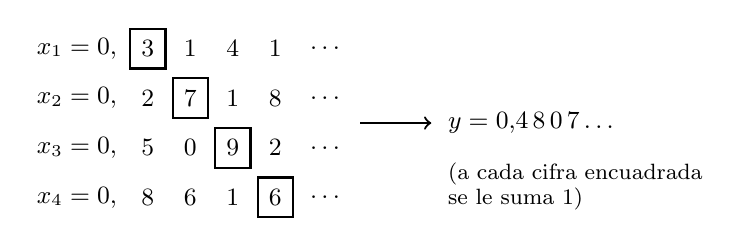
\begin{tikzpicture}[scale=0.9, every node/.style={font=\small}]
  \node at (0,0) {$x_1 = 0{,}$};
  \node at (0,-0.7) {$x_2 = 0{,}$};
  \node at (0,-1.4) {$x_3 = 0{,}$};
  \node at (0,-2.1) {$x_4 = 0{,}$};
  \foreach \fila/\a/\b/\c/\d in {0/3/1/4/1, -0.7/2/7/1/8, -1.4/5/0/9/2, -2.1/8/6/1/6} {
    \node at (1.0,\fila) {\a}; \node at (1.6,\fila) {\b};
    \node at (2.2,\fila) {\c}; \node at (2.8,\fila) {\d};
    \node at (3.5,\fila) {$\dots$};
  }
  \draw[thick] (0.75,0.28) rectangle (1.25,-0.28);
  \draw[thick] (1.35,-0.42) rectangle (1.85,-0.98);
  \draw[thick] (1.95,-1.12) rectangle (2.45,-1.68);
  \draw[thick] (2.55,-1.82) rectangle (3.05,-2.38);
  \draw[->, thick] (4.0,-1.05) -- (5.0,-1.05);
  \node[right] at (5.1,-1.05) {$y = 0{,}4\,8\,0\,7\dots$};
  \node[right, align=left] at (5.1,-1.95)
    {\footnotesize (a cada cifra encuadrada\\[-2pt] \footnotesize se le suma 1)};
\end{tikzpicture}
\end{center}

\begin{nota}
\textbf{Cuidado al explicar.} El argumento no dice «se nos escapó un número y lo agregamos».
Dice que \emph{cualquier} lista que alguien proponga deja por fuera al menos un número, y por
eso no existe una lista completa. Si alguien responde «pues lo metemos al final», hay que
celebrar la pregunta y rehacer el argumento con la lista nueva: vuelve a salir otro.
\end{nota}

\begin{nota}
\textbf{Si sobra tiempo.} La consecuencia más bonita: como $\mathbb{Q}$ se puede poner en fila
y $\mathbb{R}$ no, casi todos los reales son irracionales. Los números que sabemos nombrar
—fracciones, raíces, $\pi$, $e$— son la excepción, no la regla.
\end{nota}

\end{document}
